\section{Diagramme d'interaction : connexion}
\begin{figure}[H]
	\centering
	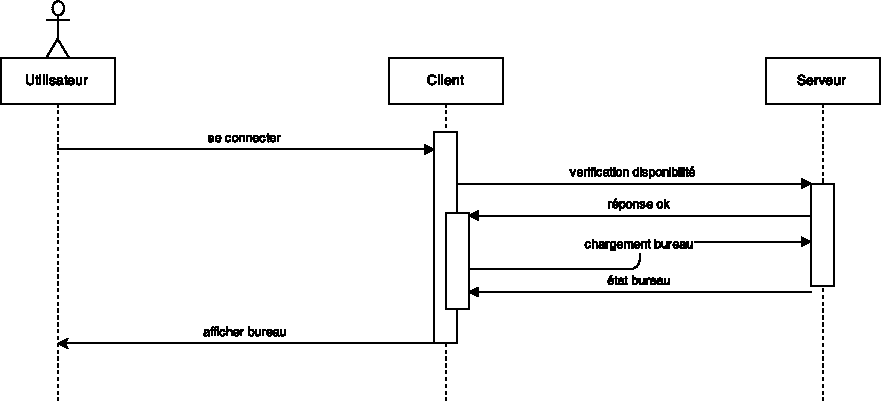
\includegraphics[angle=90]{diagrammes/DI1.pdf}
	\caption{Diagramme d'interaction : connexion}
\end{figure}

\section{Diagramme d'interaction : déplacement de widget}
\begin{figure}[H]
	\centering
	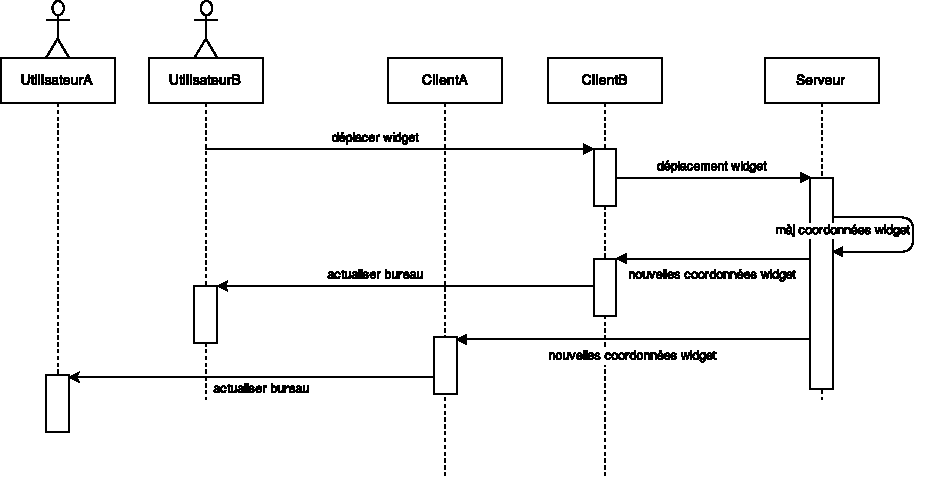
\includegraphics[angle=90]{diagrammes/DI2.pdf}
	\caption{Diagramme d'interaction : déplacement de widget}
\end{figure}

\section{Diagramme d'interaction : déplacement de widget avec conflit}
\begin{figure}[H]
	\centering
	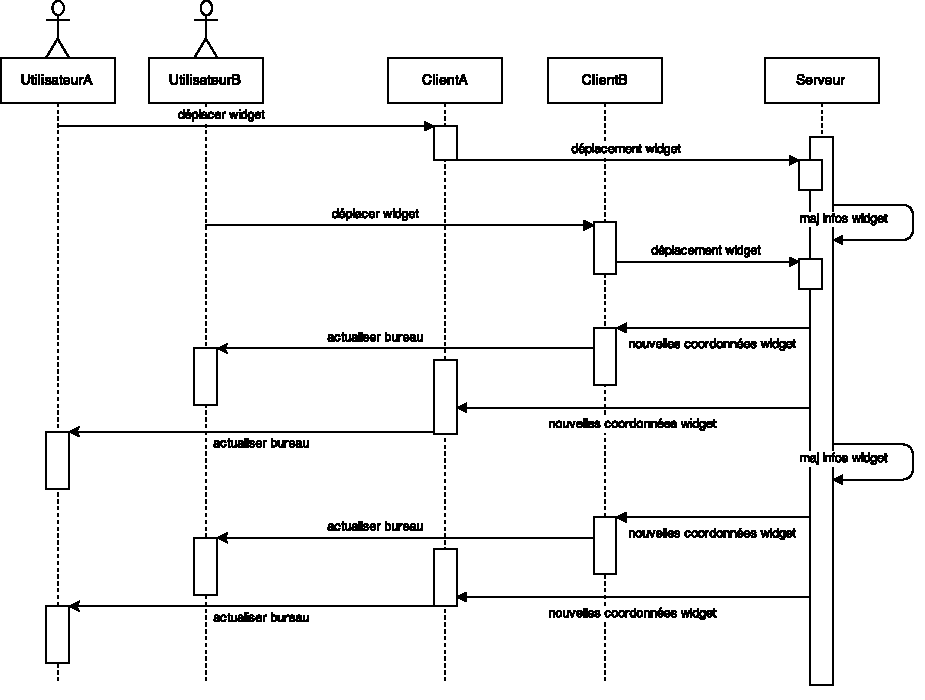
\includegraphics[angle=90]{diagrammes/DI3.pdf}
	\caption{Diagramme d'interaction : déplacement de widget avec conflit}
\end{figure}

On voit ici que lorsqu'un utilisateur prend la main sur un widget, son état ne peut être modifié par un autre utilisateur.